\newpage
\section{Angles in a Funky Shape} 

We are going to investigate the sum of the interior angles of a
funky shape.

\begin{prob}
Using a protractor, measure the interior angles of the crazy shape below:
\[
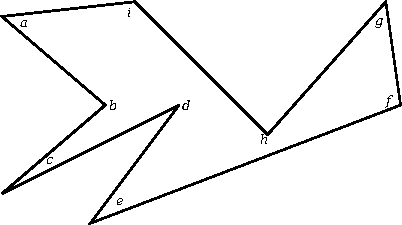
\includegraphics{../graphics/funkyshape.pdf}
\]
Use this table to record your findings:
\[
{\renewcommand{\arraystretch}{1.5}
\begin{array}{|c|c|c|c|c|c|c|c|c|}\hline
a & b & c & d & e & f & g & h & i \\\hline
\rule[7mm]{10mm}{0mm}  & \rule[7mm]{10mm}{0mm}    & \rule[7mm]{10mm}{0mm}   & \rule[7mm]{10mm}{0mm}   &  \rule[7mm]{10mm}{0mm}   & \rule[7mm]{10mm}{0mm}    & \rule[7mm]{10mm}{0mm}   & \rule[7mm]{10mm}{0mm}   & \rule[7mm]{10mm}{0mm}   \\ \hline
\end{array}}
\]
\end{prob}

\begin{prob}
Find the sum of the interior angles of the polygon above. 
\end{prob}


\begin{prob}
What should the sum be? Explain your reasoning. 
\end{prob}


